% Kopfzeile beim Kapitelanfang:
\fancypagestyle{plain}{
%Kopfzeile links bzw. innen
\fancyhead[L]{\Large Vorlesung 8 (07.11.2013)}
%Kopfzeile rechts bzw. außen
\fancyhead[R]{}}
%Kopfzeile links bzw. innen
\fancyhead[L]{\Large Vorlesung 8 (07.11.2013)}
%Kopfzeile rechts bzw. außen
\fancyhead[R]{}
% **************************************************
\subsection*{Beweise der Rechenregeln}
\en{
\item $|a_n+b_n-(a+b)| \underset{\text{Dreiecksungl.}}{\le} |a_n-a|+|b_n-b| =: s_n$\\
Zu $\eps > 0$ wähle $n_n \in \N$ so groß, dass $|a_n-a| < \frac{\eps}{2}, |b_n-b| < \frac{\eps}{2} \forall n \ge n_0$ \qed
\item In der Übung.
\item Wegen (2) o.E.: $a_n = a = 1 \forall n$\\
$|b| > 0$ und $b_n \to b \Ra \exists N \in \N: |b_n-b| < \frac{|b|}{2} \forall n \ge N$\\
$n \ge N \Ra |b_n| = |b-(b-b_n)| \underset{\text{umgk. Dreiecksungl.}}{\ge} |b|-|b-b_n| > \frac{|b|}{2}$\\
Ferner: $\left|\frac{1}{b_n} - \frac{1}{b} \right| = \frac{|b-b_n|}{|b_n| \cdot |b|} \le \frac{1}{|b|} \cdot \frac{2}{|b|} \cdot |b-b_n| \forall n \ge N$\\
Sei $\eps > 0: b_n \to b \Ra \exists n_0 \ge N: |b-b_n| < \frac{|b|^2}{2} \cdot \eps \forall n \ge n_0$\\
$\Ra \left|\frac{1}{b_n} - \frac{1}{b}\right| < \eps \forall n \ge n_0$ \qed
\item Sei $|a_n-a| < \eps \forall n \ge n_0 \Ra ||a_n|-|a|| \underset{\text{umgk. Dreiecksungl.}}{\le} |a_n-a| < \eps \forall n \ge n_0$ \qed
}

\section{Satz: Vergleichskriterium, Sandwich-Regel}\label{5.8}
\en{
\item Seien $(a_n), (b_n) \subseteq \R$ Folgen mit $a_n \to a, b_n \to b$ und $a_n \le b_n \forall n \in \N$. Dann gilt: $a \le b$
\item Speziell: Sei $a_n \to a, A \le a_n \le B \forall n \Ra A \le a \le B$
\item Seien $(a_n),(c_n) \subseteq \R$ Folgen mit $a_n \le c_n \forall n \in \N$ und $lim_{n \to \infty} a_n = a = \lim_{n \to \infty} c_n$\\
Sei $(b_n) \subseteq \R$ eine weitere Folge mit $a_n \le b_n \le c_n \forall n$\\
$\Ra (b_n)$ ist konvergent und $\lim_{n \to \infty} b_n = a$\\
$\Ra a_n \to a, c_n \to a, a_n \le b_n \le c_n \Ra b_n \to a$
}

\subsection*{Bemerkung}
Die Bedingung ``$\forall n \in \N$'' kann überall ersetzt werden durch ``$\forall n \in \N$ mit $n \ge N$'', $N \in \N$ geeignet.

\subsection*{Beispiel}
$x > 0 \Ra$ \fbox{$\sqrt[n]{x} \to 1 \text{ für } n \to \infty$}\\
Denn: o.E. $x > 1$, denn $x=1$ klar, falls $x < 1$ betrachte $\frac{1}{x} > 1$\\
$\Ra 1 < \sqrt[n]{x} < \underbrace{\sqrt[n]{n}}_{1}$ für $n > x$\\
Dank Sandwich-Regel folgt die Behauptung. \qed

\subsection*{Beweis von 5.8}
\en{
\item Angenommen, $a>b$. Setze $\eps := a-b > 0$\\
$\Ra \exists n_0 \in \N: |a_n-a| < \frac{\eps}{3}, |b_n-b| < \frac{\eps}{3} \forall n \ge n_0$\\
$\Ra 0 \le b_n-a_n = \underbrace{(b_n-b)}_{< \frac{\eps}{3}} + \underbrace{(b-a)}_{- \eps} + \underbrace{(a-a_n)}_{< \frac{\eps}{3}} < - \frac{\eps}{3} < 0$ \wspruch
\item Ausgelassen
\item $|b_n-a| = |b_n-a_n+a_n-a| \underset{\text{Dreiecksungl.}}{\le} (b_n-a_n)+|a_n-a| \le \underbrace{(c_n-a_n)}_{\to 0} + \underbrace{|a_n-a|}_{\to 0} =: s_n$\\
$\Ra s_n \to 0$ (alles nach Regeln 5.7)\\
Sei $\eps > 0 \Ra \exists n_0 \in \N: s_n < \eps \forall n \ge n_0 \Ra |b_n-a| < \eps \forall n \ge n_0$ \qed
} 

\section{Definition: Monotone Folgen}\label{5.9}
Sei $(a_n) \subseteq \R$ eine Folge.
\enr{
\item $(a_n)$ ist monoton wachsend $\Lra a_{n+1} \ge a_n \forall n \in \N$\\
$(a_n)$ ist monoton fallend $\Lra a_{n+1} \le a_n \forall n \in \N$
\item Ist dabei stets $a_{n+1} > a_n$ bzw. $a_{n+1} < a_n$, so spricht man von strenger Monotonie
\item $(a_n) \subseteq \R$ ist monton, falls $(a_n)$ monoton wachsend oder fallend ist
}

\subsection*{Beispiele}
\items{
\item $a_n = n^2$ ist streng monoton wachsend
\item $a_n = \frac{1}{n}$ ist streng monoton fallend
\item $a_n = -n$ ist streng monoton fallend
\item $a_n = (-1)^n \cdot n$ ist nicht monoton
}

\section{Monotoniekriterium}\label{5.10}
Jede monotone \underline{und} beschränkte Folge ist konvergent.\\
Dabei gilt: $\lim_{n \to \infty} a_n = \left\{\begin{array}{l l}
\sup\{a_n: n \in \N\} & \text{falls } (a_n) \text{ monoton wachsend}\\
\inf\{a_n: n \in \N\} & \text{falls } (a_n) \text{ monoton fallend}
\end{array} \right.$

\subsection*{Beweis (für wachsend)}
$s := sup\{a_n: n \in \N\}$ existiert, da $(a_n)$ beschränkt ist.\\
Sei $\eps > 0 \Ra \exists n_0 \in \N: a_{n_0} > s-\eps$\\
Monotonie von $(a_n) \Ra s-\eps < a_{n_0} \le a_n \le s \forall n \ge n_0$\\
$\Ra |a_n-s| < \eps \forall n \ge n_0$ \qed

\subsection*{Bemerkung}
Es genügt, dass $(a_n)$ monoton ab einem gewissen Index $N \in \N$ ist.

\newpage

\section{Beispiel: Babylonisches Wurzelziehen}\label{5.11}
\emph{Algorithmus zur Berechnung von $\sqrt{a}, a > 0$}\nl
Motivation: Sei $\xi > 0$  (sprich: ``\emph{xi}'') eine Näherung für $\sqrt{a}$.\\
Angenommen, $\xi > \sqrt{a} \Ra \frac{a}{\xi} < \sqrt{a}$\\
Betrachte $\frac{1}{2} \cdot \left(\xi + \frac{a}{3}\right)$ als neue Näherung!\\
Definiere rekursiv Näherungen $x_n, n \in \N_0$:\\
$x_0 > 0$ beliebig, z.B. $x_0 = a$\\
$\forall n \in \N_0: x_{n+1} := \frac{1}{2} \cdot \left(x_n + \frac{a}{x_n}\right)$

\subsection*{Behauptung}
$x_n \to \sqrt{a}$

\subsection*{Beweis}
Induktion zeigt: $x_n > 0 \forall n \ge 0$.\\
Ferner: $x_{n+1}^2 - a = \frac{1}{4} \cdot \left(x_n + \frac{a}{x_n}\right) - a = \frac{1}{4} \cdot \left(x_n^2 + 2a + \frac{a^2}{x_n^2} - 4a \right) = \frac{1}{4} \cdot \left(x_n - \frac{a}{x_n}\right)^2 \ge 0$\\
$\underset{x_n > 0}{\Ra} x_n \ge \sqrt{a} \forall n \in \N$

\subsection*{Behauptung}
$(x_n)_{n \ge 1}$ ist monoton fallend (und dank obigem Beweis auch beschränkt).\\
Monotoniekriterium $\Ra x = \lim_{n \to \infty} x_n$ existiert, und $x \ge \sqrt{a}$ (Vergleichskriterium)

\subsection*{Frage}
Was ist der Grenzwert $x$? Betrachte Rekursion!\\
$\underbrace{x_{n+1}}_{\to x} = \underbrace{\frac{1}{2} \cdot \left(x_n + \frac{a}{x_n}\right)}_{\to \frac{1}{2} \cdot \left(x + \frac{a}{x}\right)}$\\
$\Ra x = \frac{1}{2} \cdot \left(x + \frac{a}{x}\right) \Lra x^2 = a \underset{x > 0}{\Ra} x = \sqrt{a}$

\subsection*{Beobachtung}
Das Verfahren konvergiert sehr schnell.

\newpage

\phantomsection
\addcontentsline{toc}{section}{Teilfolgen}
\section*{Teilfolgen}\label{Teilfolgen}
Sei $X$ eine Menge, $(a_n)_{n \in \N} \subseteq X$ eine Folge in $X$.\\
Ist $n_1 < n_2 < n_3 < \hdots < n_k < \hdots$ eine aufsteigende Folge von Indizes $n_k \in \N$, so heißt $(a_{n_k})_{k \in \N} = (a_{n_1}, a_{n_2}, \hdots)$ eine Teilfolge von $(a_n)$.\\
Ist $J=\{n_k: k \in \N\}$, so schreiben wir auch $(a_j)_{j \in J}$.

\subsection*{Beispiel}
$(a_p)_{p \text{ prim}} = (a_2, a_3, a_5, a_7, a_{11}, \hdots)$

\subsection*{Bemerkung}
Ist $(a_n)_{n \in \N}$ konvergent mit Grenzwert $a \Ra$ Jede Teilfolge von $(a_n)$ konvergiert ebenfalls gegen $a$: $\lim_{n \to \infty} a_{n_k} = a$

\section{\texorpdfstring{Satz von Bolzano-Weierstraß in $\R$}{Satz von Bolzano-Weierstraß in \R}}\label{5.12}
Jede beschränkte Folge $(a_n)_{n \in \N} \subseteq \R$ besitzt eine konvergente Teilfolge.

\subsection*{Beweis}
Wir zeigen: $(a_n)$ enthält eine monotone Teilfolge.\\
Mit dem Monotoniekriterium ist diese Teilfolge konvergent.\nl
Wir definieren dazu: $J := \{j \in \N: a_j \ge a_n \forall n > j\}$\\
Das heißt: $j \in J \Lra$ alle Folgenglieder ab dem $j$-ten Glied sind $\le a_j$.\nl
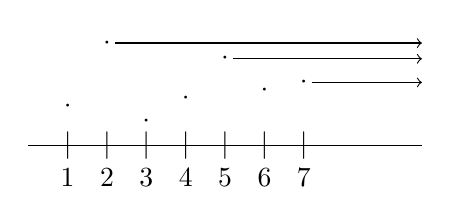
\begin{tikzpicture}
\draw(0,0)--(5,0);
\foreach \x/\xtext in {0.5/$1$,1.0/$2$,1.5/$3$,2.0/$4$,2.5/$5$,3.0/$6$,3.5/$7$}
  \draw(\x,0pt) node{$|$} (\x,-5pt) node[below] {\xtext};
\draw(0.5,0.5) node{$\cdot$};
\draw(1.0,1.3) node{$\cdot$};
\draw[->](1.1,1.3)--(5.0,1.3);
\draw(1.5,0.3) node{$\cdot$};
\draw(2.0,0.6) node{$\cdot$};
\draw(2.5,1.1) node{$\cdot$};
\draw[->](2.6,1.1)--(5.0,1.1);
\draw(3.0,0.7) node{$\cdot$};
\draw(3.5,0.8) node{$\cdot$};
\draw[->](3.6,0.8)--(5.0,0.8);
\end{tikzpicture}
$J = \{2,5,7,\hdots\}, (a_j)_{j \in J} = (a_2, a_5, a_7, \hdots)$
\begin{enumerate}[label=\arabic*. Fall:]
\item $J$ nach oben unbeschränkt $\Ra (a_j)_{j \in J}$ ist monoton fallende Teilfolge
\item $J$ ist nach oben beschränkt, etwa durch $m \in \N$.\\
Dann gilt: (*) $\forall j>m \exists n>j$ mit $a_n > a_j$.\\
Konstruiere mittels (*) rekursiv eine monoton wachsende Teilfolge $(a_{n_k})_{k \in \N}$:\\
$n_1 := m+1$\\
(*) mit $j=n_1$: $\exists n_2 > n_1: a_{n_2} > a_{n_1}$\\
(*) mit $j=n_2$: $\exists n_3 > n_2: a_{n_3} > a_{n_2}$\\
$\hdots$\\
Wir erhalten also eine monoton wachsende Folge.
\end{enumerate} \qed